\documentclass[tikz,border=4pt]{standalone}
\usepackage{lmodern}
\usetikzlibrary{arrows.meta,positioning,fit,backgrounds}
\definecolor{ink}{HTML}{0B0B0B}
\definecolor{ink2}{HTML}{52514E}
\definecolor{edge}{HTML}{898781}
\definecolor{accent}{HTML}{2A78D6}
\definecolor{tint}{HTML}{F0EFEC}
\begin{document}
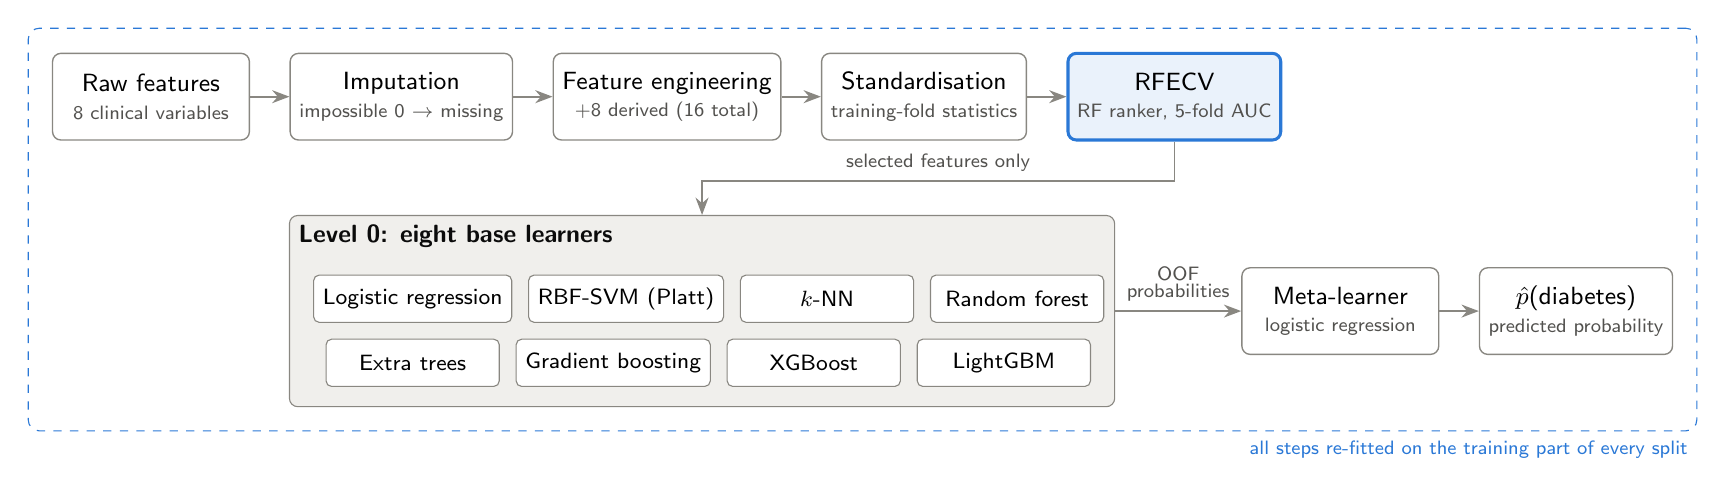
\begin{tikzpicture}[
  font=\sffamily\small,
  >={Stealth[length=2.2mm]},
  stage/.style={draw=edge, rounded corners=3pt, align=center, minimum width=25mm, minimum height=11mm, line width=0.5pt},
  key/.style={stage, draw=accent, line width=1.1pt, fill=accent!10},
  chip/.style={draw=edge, rounded corners=2pt, minimum width=22mm, minimum height=6mm, font=\sffamily\footnotesize, fill=white},
  sub/.style={font=\sffamily\scriptsize, text=ink2},
  arr/.style={->, draw=edge, line width=0.6pt}
]
\node[stage] (raw) {Raw features\\[-1pt]{\scriptsize\color{ink2} 8 clinical variables}};
\node[stage, right=5mm of raw] (imp) {Imputation\\[-1pt]{\scriptsize\color{ink2} impossible 0 $\to$ missing}};
\node[stage, right=5mm of imp] (eng) {Feature engineering\\[-1pt]{\scriptsize\color{ink2} +8 derived (16 total)}};
\node[stage, right=5mm of eng] (sca) {Standardisation\\[-1pt]{\scriptsize\color{ink2} training-fold statistics}};
\node[key, right=5mm of sca] (rfe) {RFECV\\[-1pt]{\scriptsize\color{ink2} RF ranker, 5-fold AUC}};
\foreach \a/\b in {raw/imp, imp/eng, eng/sca, sca/rfe} \draw[arr] (\a) -- (\b);

\node[chip, below=17mm of imp.south west, anchor=north west, xshift=3mm] (c1) {Logistic regression};
\node[chip, right=2mm of c1] (c2) {RBF-SVM (Platt)};
\node[chip, right=2mm of c2] (c3) {$k$-NN};
\node[chip, right=2mm of c3] (c4) {Random forest};
\node[chip, below=2mm of c1] (c5) {Extra trees};
\node[chip, right=2mm of c5] (c6) {Gradient boosting};
\node[chip, right=2mm of c6] (c7) {XGBoost};
\node[chip, right=2mm of c7] (c8) {LightGBM};
\begin{scope}[on background layer]
  \node[draw=edge, fill=tint, rounded corners=3pt, inner xsep=3mm, inner ysep=5mm, yshift=2.5mm, fit=(c1)(c8), label={[anchor=north west, font=\sffamily\small\bfseries, text=ink]north west:Level 0: eight base learners}] (lvl0) {};
\end{scope}
\node[stage, right=16mm of lvl0] (meta) {Meta-learner\\[-1pt]{\scriptsize\color{ink2} logistic regression}};
\node[stage, right=5mm of meta, minimum width=20mm] (out) {$\hat p$(diabetes)\\[-1pt]{\scriptsize\color{ink2} predicted probability}};
\draw[arr] (rfe.south) -- ++(0,-5mm) -| node[pos=0.25, above, sub] {selected features only} (lvl0.north);
\draw[arr] (lvl0) -- node[above, sub, align=center] {OOF\\[-2pt]probabilities} (meta);
\draw[arr] (meta) -- (out);

\node[draw=accent, dashed, rounded corners=4pt, inner sep=3mm, fit=(raw)(rfe)(lvl0)(out), label={[font=\sffamily\scriptsize, text=accent, anchor=north east]south east:all steps re-fitted on the training part of every split}] {};
\end{tikzpicture}
\end{document}
